There are four ways to install \app{} (Table~\ref{tab:install}). Most users should
use the portable package.

\subsection{Requirements}

\begin{table}[H]
  \centering
  \caption{Installation options}
  \label{tab:install}
  \begin{tabularx}{\textwidth}{l l L}
    \toprule
    \textbf{Option} & \textbf{Platform} & \textbf{Needs} \\
    \midrule
    Portable package (recommended) & Windows 10/11, x64 & Nothing else. Python and all libraries are included; no internet connection or administrator rights are needed. \\
    Source installer & Windows & Internet access during the first run, to download the \texttt{uv} package manager, Python and the libraries. \\
    Source installer & Linux & The same, run from a terminal. \\
    From source & Any & \texttt{uv}~\cite{uv} and a copy of the repository. \\
    \bottomrule
  \end{tabularx}
\end{table}

Once installed, \app{} works offline.

\subsection{Portable Windows Package (Recommended)}

The portable package is a ZIP file containing the tool, Python, the libraries and the
12 one-line layouts provided with the project. It needs no installation and changes no
system settings, so it suits company computers where installing software is
restricted.

\begin{enumerate}
  \item Copy \texttt{GFT\_Analysis\_Tool-Windows-Portable.zip} to the computer.
  \item Right-click it, choose \menu{Extract All}, and extract it to a folder you can
        save files in.
  \item Open the extracted \code{GFT_Analysis_Tool_Portable} folder and
        double-click \code{GFT_Analysis_Tool.exe}.
\end{enumerate}

\begin{note}
Keep the \texttt{\_internal} folder next to the executable, and do not run the program
from inside the ZIP. The package is not code-signed, so your organization's security
policy may block it. If it does, ask IT to approve it rather than working around the
block.
\end{note}

The extracted folder also contains:
\begin{itemize}
  \item the layouts, in \texttt{One-Line Layouts};
  \item launch instructions;
  \item \texttt{BUILD INFO.json}, which records the tool's version and the library
        versions;
  \item a checksum file for the ZIP;
  \item the source code and the libraries' license notices.
\end{itemize}

\paragraph{Building the package.} A developer builds the package on a Windows
computer with PyInstaller~\cite{pyinstaller}, by running these commands in the
repository:

\begin{lstlisting}
uv sync --locked --group package
.venv\Scripts\python.exe install\build_portable.py
\end{lstlisting}

The result is \texttt{dist\textbackslash GFT\_Analysis\_Tool-Windows-Portable.zip}.

\paragraph{Updating.} Each new version is a new ZIP. Delete the old folder and extract
the new one. Your layouts and reports are saved elsewhere, so they are not affected.

\subsection{Windows Source Installer}

\begin{enumerate}
  \item Extract the project ZIP with \menu{Extract All} into the folder where it will
        stay. The desktop shortcut points to this folder, so do not move it afterward.
  \item Open the \texttt{install} folder and double-click \texttt{install.bat}.
  \item If Windows shows ``Windows protected your PC'', choose \menu{More info} and
        then \menu{Run anyway}, if your organization allows it.
  \item Wait until the window shows \emph{Setup Complete!} The first run downloads
        Python and the libraries, which can take a few minutes.
  \item Start the tool from the new \textbf{\app{}} shortcut on the desktop.
\end{enumerate}

\subsection{Linux}

Extract the project, open a terminal in the project folder and run:

\begin{lstlisting}
bash install/install.sh
\end{lstlisting}

This installs the libraries and adds \app{}, with the GFT icon, to the applications
menu and the desktop. It is safe to run again.

\subsection{Running from Source}

With \texttt{uv} installed, run from the project folder:

\begin{lstlisting}
uv sync --locked
uv run gft-opto
\end{lstlisting}

The \texttt{--locked} option installs exactly the library versions listed in
\texttt{uv.lock}, so every installation behaves the same.

\subsection{First Launch}

\app{} opens full-screen with an empty drawing named \emph{Untitled Project}
(Figure~\ref{fig:startup}). The Equipment Library starts empty; you add equipment with
\ui{Create Component} or by opening a layout. Section~\ref{sec:quickstart} continues
from here.


\begin{figure}[H]
  \centering
  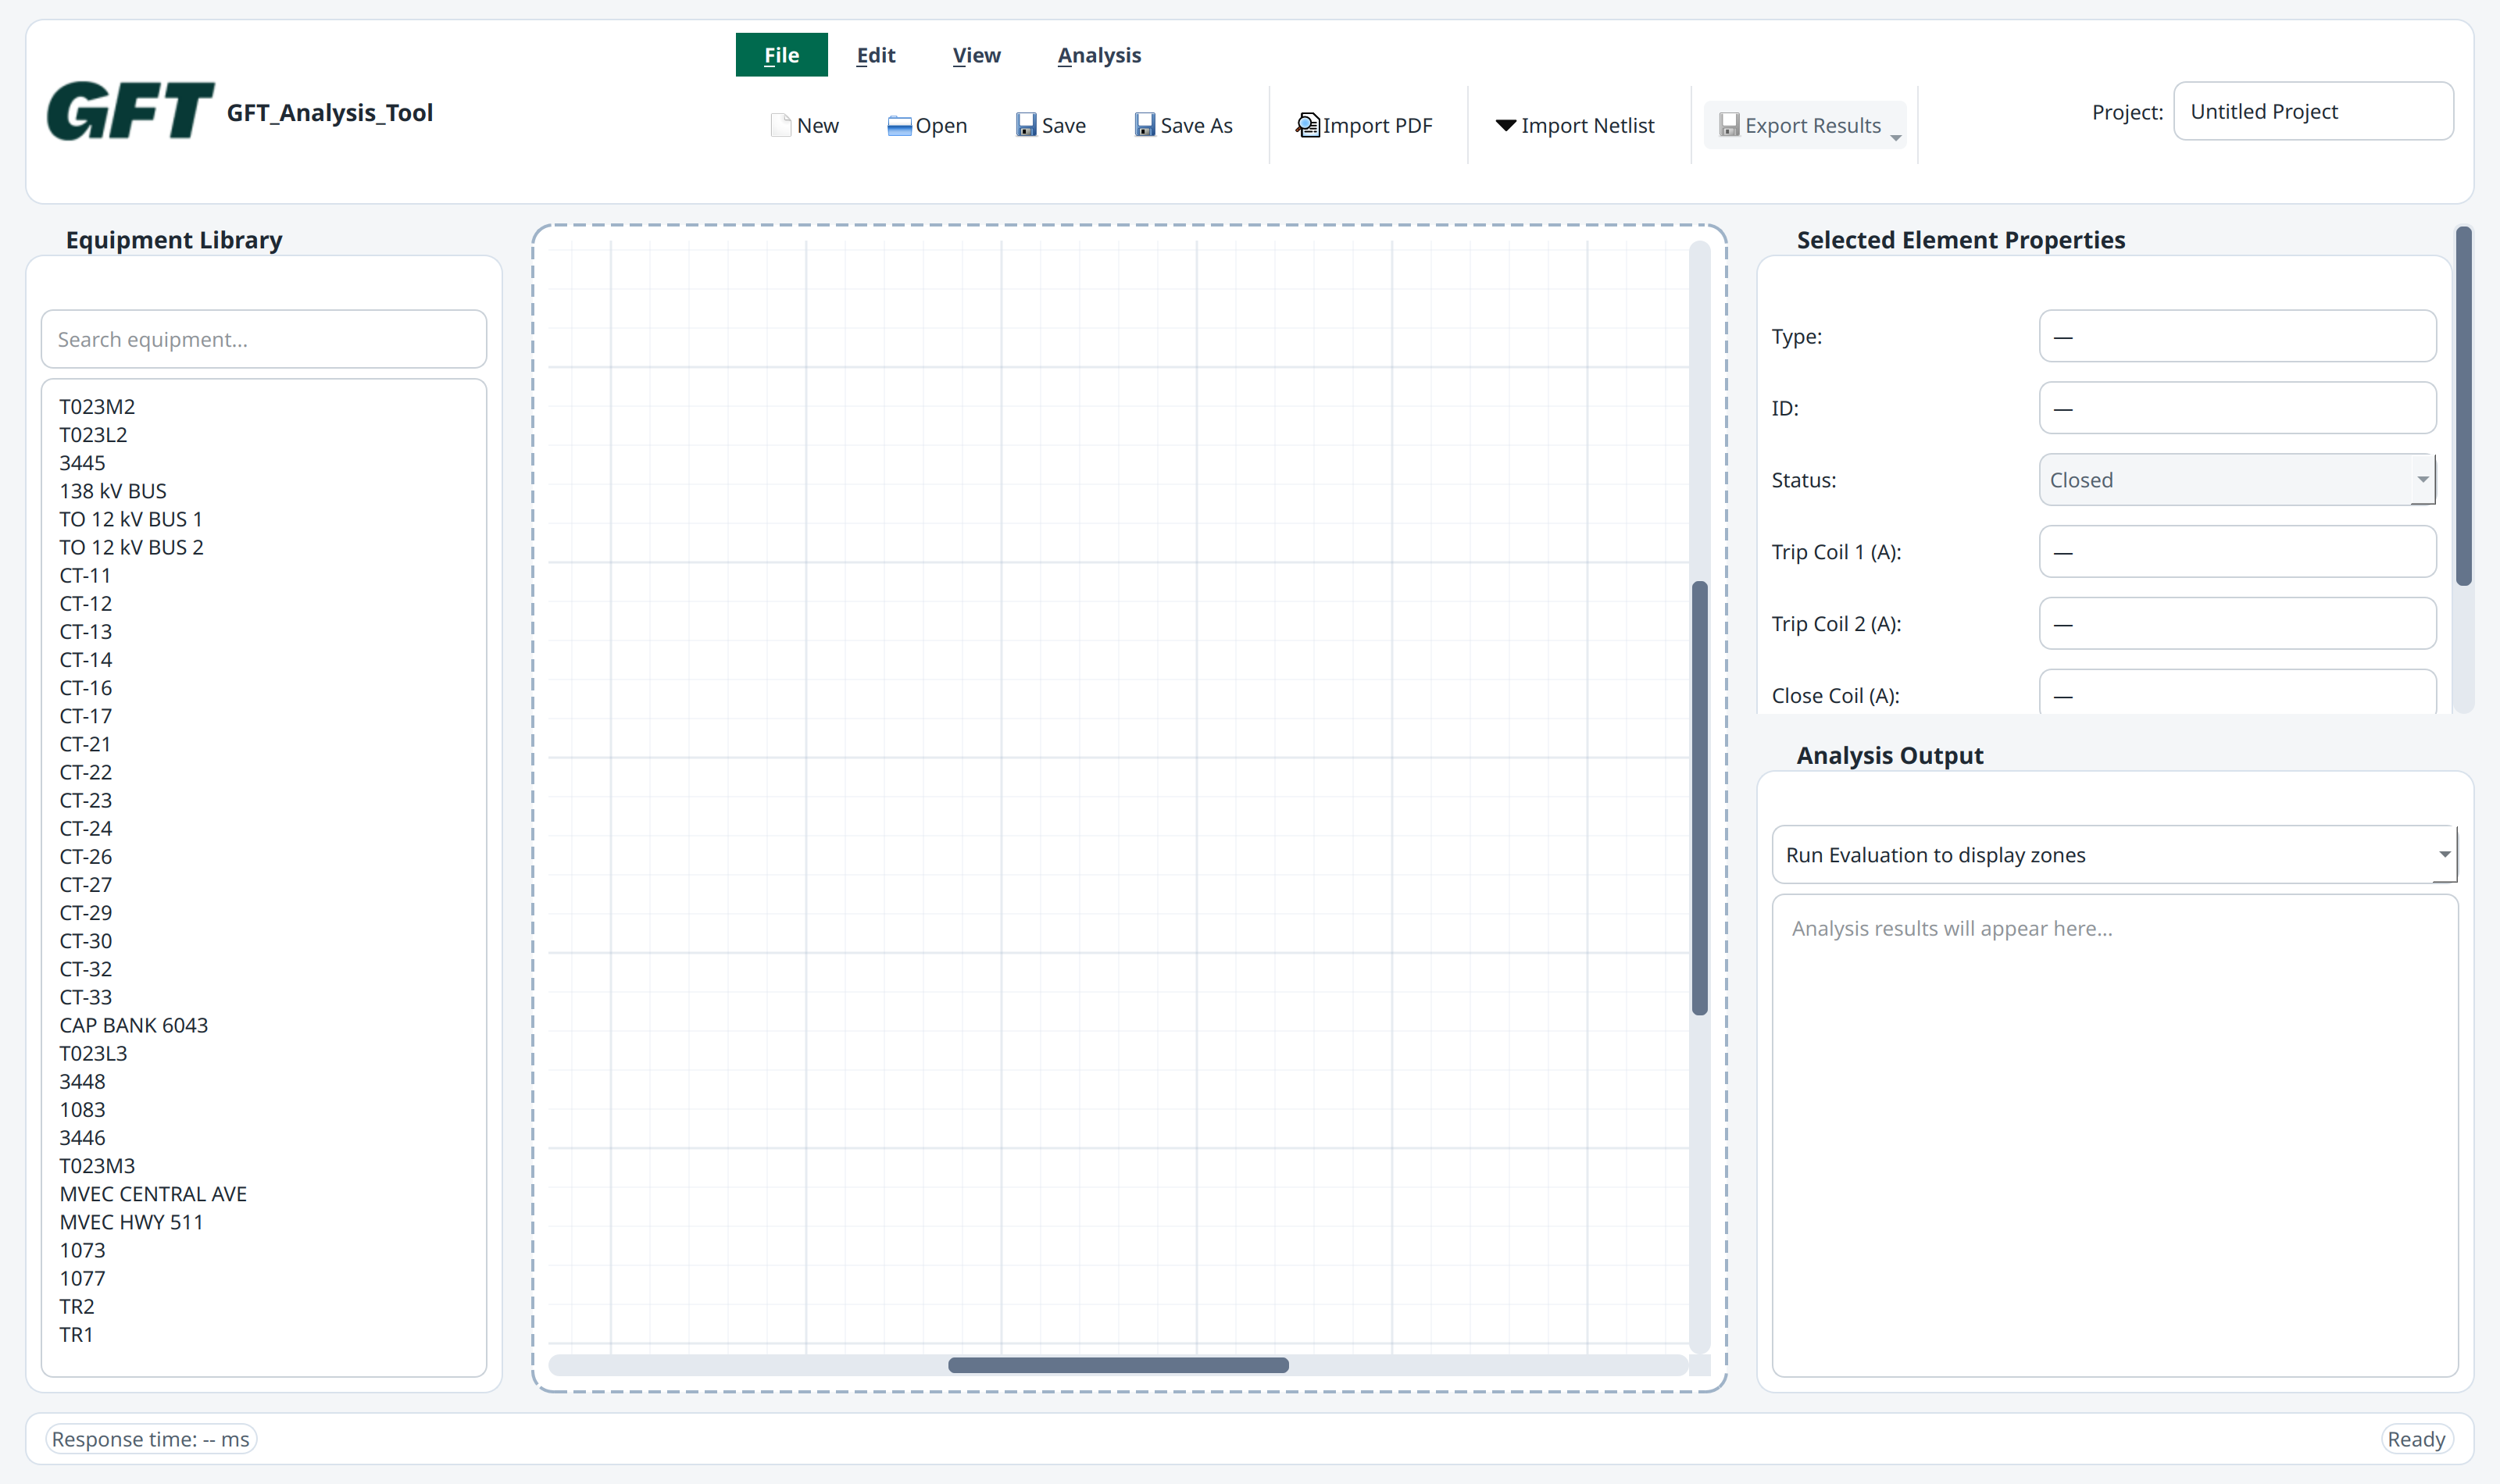
\includegraphics[width=0.85\textwidth]{images/startup_window.png}
  \caption{\app{} at start-up}
  \label{fig:startup}
\end{figure}
